\documentclass{article}
\usepackage{graphicx} % Required for inserting images
\usepackage[utf8]{inputenc}
\usepackage{polski}
\usepackage[dvipsnames]{xcolor}
\usepackage{indentfirst}
\usepackage{multicol}
\usepackage{geometry}
\usepackage{titlesec}
\usepackage[colorlinks=true, linkcolor=gray, urlcolor=blue, citecolor=green]{hyperref}
\usepackage{makecell}
\usepackage{float}
\usepackage[polish]{babel}
\usepackage[T1]{fontenc}
\usepackage[justification=centering]{caption}
\usepackage[utf8]{inputenc} 
\usepackage{subfig}


\usepackage{mwe} % for 'example-image'
\usepackage{newfloat}
\DeclareFloatingEnvironment{graph}
\addto\captionspolish{%
  \renewcommand{\graphname}{Wykres}%
  \renewcommand{\figurename}{Rysunek}%
  \renewcommand{\tablename}{Tabela}%
}


\begin{document}

\begin{titlepage}
    \begin{center}
        \vspace*{1cm}
            
        \Huge
        \textbf{Sprawozdanie z laboratorium 5}
            
        \vspace{0.5cm}
        \LARGE
        IO-LINK (S7-1200) 
            
        \vspace{1.5cm}
            
        \textbf{Łukasz Janusz\\Marek Generowicz}

        \normalsize      
        \textcolor{gray}{13.03.2025}
        \vfill
        \begin{figure}[hb]
            \centering
            
\includegraphics[width=0.5\textwidth]{media/Logo_AGH.jpg}
        \end{figure}   
    \end{center}
\end{titlepage}

\section{Wstęp}
Na laboratoriach należało zapoznać się z protokołem HART, zasadami komunikacji oraz praktycznymi aspektami wykorzystania go w przemyśle. W trakcie zajęć przeprowadzono ćwiczenia z wykorzystaniem sterownika \textit{WAGO 750-841} wyposażonym w dwukanałowy analogowy moduł wejścia, który pozwala na komunikację z urządzeniami HART. Elementem pomiarowym natomiast jest \textit{termopara typu K}, która została połączona z modułem WAGO za pomocą przetwornika temperatury \textit{TxIsoRail-HART}. 
\vspace{1em}
\begin{figure}[ht]
    \centering
    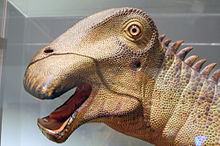
\includegraphics[width=1\linewidth]{media/Brak_zdjecia.png}
    \caption{Program obsługujący wejście analogowe modułu HART.}
    \label{fig2}
\end{figure}
\vspace{2em}
\end{document}
